\section{Metaheuristic Optimization Algorithms II}
Advanced applications of metaheuristic algorithms and hybrid approaches will be examined in this section. Modern techniques used in solving optimization problems and their applications will be discussed.

\subsection{Simulated Annealing (SA)}
Simulated Annealing (SA) is a powerful metaheuristic optimization algorithm inspired by the annealing process in metallurgy. In the annealing process of metals, the material is first heated to high temperatures, during which atoms move randomly at high energy levels. Then, the material is slowly cooled in a controlled manner, allowing atoms to settle into a low-energy, stable crystal structure. This physical process has been adapted as an effective strategy for reaching the global optimum in optimization problems. The algorithm accepts poor solutions with a certain probability at the beginning with a high "temperature" parameter, thus exploring a wide search space. As the temperature gradually decreases, the algorithm becomes more selective and performs more intensive search in promising regions. This approach reduces the risk of getting stuck in local optima and increases the probability of converging to the global optimum in complex and multimodal optimization problems.\sidenote{Simulated annealing provides successful results especially in combinatorial optimization problems. The cooling rate and initial temperature are important parameters affecting the algorithm's performance. Example Python code implementing the simulated annealing algorithm on the Ackley function:

\qrcode[height=1in]{https://github.com/btayfur/structural-optimization/blob/main/Code/Examples/Exmp1}}

\subsubsection{Algorithm Basis}
An optimization algorithm inspired by the annealing process of metals:
\begin{itemize}
    \item Random movements at high temperature
    \item Controlled movements as temperature decreases
    \item Probability of accepting poor solutions
\end{itemize}

\begin{equation}
P(\Delta E) = \exp\left(-\frac{\Delta E}{kT}\right)
\end{equation}

\begin{figure}[h]
\centering
\begin{tikzpicture}
\draw[->] (0,0) -- (4,0) node[right] {Iteration};
\draw[->] (0,0) -- (0,4) node[above] {Temperature};
\draw[scale=1,domain=0:4,smooth,variable=\x,blue] 
    plot ({\x},{3*exp(-0.5*\x)});
\end{tikzpicture}
\caption{Temperature change in simulated annealing}
\label{fig:sa_temp}
\end{figure}

\subsubsection{Algorithm Steps}
\begin{enumerate}
    \item Determine initial temperature and solution
    \item For each temperature level:
        \begin{itemize}
            \item Generate new solution
            \item Calculate energy difference
            \item Accept/reject according to Metropolis criterion
        \end{itemize}
    \item Decrease temperature
    \item Continue until stopping criterion is met
\end{enumerate}

\subsection{Tabu Search Algorithm}
The Tabu Search Algorithm (TS), developed by Fred Glover in 1986, is a powerful metaheuristic optimization method inspired by human memory. It mimics the human intelligence's ability to benefit from past experiences and prevent repeating errors in the problem-solving process. The algorithm provides effective results especially in combinatorial optimization problems and is designed to overcome the local optima trapping problem of local search methods. Tabu Search gets its name from the tabu list, which is the algorithm's fundamental component and temporarily "forbids" recently visited solutions. This approach prevents the search process from repeatedly visiting the same solutions, enabling exploration of wider regions of the search space.

The Tabu Search Algorithm works by systematically evaluating potential solutions in the neighborhood of the current solution. In each iteration, all solutions (or a specific subset) in the neighborhood of the current solution are examined, and the best solution not in the tabu list is selected. The move corresponding to the selected solution is added to the tabu list, and the list forbids this move for a certain period (tabu tenure). However, even a move in the tabu list can be accepted if it satisfies certain conditions known as the "aspiration criterion" (for example, if it produces a better solution than the best solution found so far). The algorithm also uses "intensification" (more detailed search in promising regions) and "diversification" (moving to different regions of the search space) strategies to guide the search process. This balanced approach enables the algorithm to both effectively investigate local optima and increase the probability of converging to the global optimum.

\subsubsection{Basic Concepts}
\begin{itemize}
    \item Tabu list
    \item Neighborhood structure
    \item Aspiration criterion
    \item Intensification and diversification
\end{itemize}

\begin{tcolorbox}[title=Role of Tabu List]
\begin{itemize}
    \item Stores recently visited solutions
    \item Prevents cyclic movements
    \item Explores different regions of search space
    \item List length is an important parameter
\end{itemize}
\end{tcolorbox}

\subsubsection{Algorithm Steps}
\begin{enumerate}
    \item Determine initial solution
    \item In each iteration:
        \begin{itemize}
            \item Generate neighbor solutions
            \item Check tabu list
            \item Select best suitable solution
            \item Update tabu list
        \end{itemize}
    \item Continue until stopping criterion is met
\end{enumerate}

\begin{marginfigure}
\centering
\begin{tikzpicture}
\draw[->] (0,0) -- (4,0) node[right] {$x_1$};
\draw[->] (0,0) -- (0,4) node[above] {$x_2$};
\filldraw[blue] (1,1) circle (2pt);
\filldraw[blue] (2,2) circle (2pt);
\filldraw[blue] (3,1) circle (2pt);
\draw[->,red] (1,1) -- (2,2);
\draw[->,red] (2,2) -- (3,1);
\end{tikzpicture}
\caption{Tabu search algorithm movement}
\label{fig:tabu_search}
\end{marginfigure}

\subsection{Genetic Algorithms (GA)}
Genetic Algorithms (GA), developed by John Holland in 1975, are a metaheuristic optimization method that mimics the natural evolution process. These algorithms work in the solution space and manage the search process using the genetic structures of solutions. GA has a structure where solutions are represented by chromosomes (genes) and these chromosomes are subjected to the evolution process under selected constraints.

The working principle of Genetic Algorithms is a process that mimics natural selection and genetic mechanisms. The algorithm begins by encoding potential solutions as chromosomes and creating a random initial population. In each iteration, the fitness values of solutions are calculated, and individuals with higher fitness have a greater chance of reproduction. Selected parents undergo crossover to share genetic information and create a new generation. Mutation is applied with a low probability to maintain diversity and explore different regions of the search space. This process is repeated until a certain stopping criterion is met (maximum number of generations, sufficient fitness value, etc.). The strength of Genetic Algorithms lies in their ability to converge to the global optimum even in complex and multidimensional problems and their easy adaptability to different problem types.

\subsubsection{Basic Components}
\begin{itemize}
    \item Chromosome (solution) structure
    \item Population
    \item Selection mechanism
    \item Crossover operator
    \item Mutation operator
\end{itemize}

\begin{equation}
P(x_i) = \frac{f(x_i)}{\sum_{j=1}^N f(x_j)}
\end{equation}

\sidenote{Genetic algorithms are inspired by Darwin's theory of evolution. The principle of survival of the fittest ensures the production of better solutions in the optimization process.}

\subsubsection{Algorithm Steps}
\begin{enumerate}
    \item Create initial population
    \item In each generation:
        \begin{itemize}
            \item Calculate Fitness values
            \item Select parents
            \item Apply crossover and mutation
            \item Create new generation
        \end{itemize}
    \item Continue until stopping criterion is met
\end{enumerate}

\begin{tcolorbox}[title=Genetic Operators]
\begin{itemize}
    \item \textbf{Crossover:}
        \begin{itemize}
            \item Single-point
            \item Multi-point
            \item Uniform
        \end{itemize}
    \item \textbf{Mutation:}
        \begin{itemize}
            \item Bit flip
            \item Gaussian
            \item Uniform
        \end{itemize}
\end{itemize}
\end{tcolorbox}

\subsection{Particle Swarm Optimization (PSO)}
Particle Swarm Optimization (PSO), developed by Russell Eberhart and James Kennedy in 1995, is a metaheuristic optimization method that mimics the natural evolution process. PSO represents solutions as particles and manages the search process using the effects of other particles in the swarm.

PSO is a process where particles move by benefiting from their own experience and the collective knowledge of the swarm. Each particle tracks its own best solution (pbest) and the swarm's best solution (gbest). The velocity and position of particles are updated with the effects of other particles in the swarm, thus increasing the probability of converging to the global optimum in the search space. PSO provides successful results in multidimensional and complex optimization problems and stands out with its fast convergence ability, few parameters, and easy adaptability.

\subsubsection{Basic Concepts}
\begin{itemize}
    \item Particle position and velocity
    \item Personal best (pbest)
    \item Global best (gbest)
    \item Inertia weight
    \item Learning factors
\end{itemize}

\begin{equation}
\begin{aligned}
v_{i,j}^{t+1} &= w v_{i,j}^t + c_1r_1(pbest_{i,j} - x_{i,j}^t) + c_2r_2(gbest_j - x_{i,j}^t) \\
x_{i,j}^{t+1} &= x_{i,j}^t + v_{i,j}^{t+1}
\end{aligned}
\end{equation}

\begin{marginfigure}
\centering
\begin{tikzpicture}
\draw[->] (0,0) -- (4,0) node[right] {$x_1$};
\draw[->] (0,0) -- (0,4) node[above] {$x_2$};
\filldraw[blue] (2,2) circle (2pt) node[above] {gbest};
\filldraw[red] (1,1) circle (2pt);
\draw[->,green] (1,1) -- (1.5,1.5);
\end{tikzpicture}
\caption{Particle movement in PSO}
\label{fig:pso_movement}
\end{marginfigure}

\subsubsection{Algorithm Steps}
\begin{enumerate}
    \item Initialize swarm
    \item In each iteration:
        \begin{itemize}
            \item Calculate fitness values
            \item Update pbest and gbest
            \item Update velocities and positions
        \end{itemize}
    \item Continue until stopping criterion is met
\end{enumerate}

\sidenote{PSO is inspired by the behavior of bird flocks. Particles move by benefiting from both their own experience and the collective knowledge of the swarm.}

\subsection{Advantages and Disadvantages of Algorithms}

\begin{tcolorbox}[title=Comparative Analysis]
\begin{itemize}
    \item \textbf{Simulated Annealing:}
        \begin{itemize}
            \item + Simple implementation
            \item + Theoretical convergence guarantee
            \item - Slow convergence
            \item - Sensitive parameter tuning
        \end{itemize}
    \item \textbf{Tabu Search:}
        \begin{itemize}
            \item + Avoids cyclic movements
            \item + Effective in local search
            \item - Memory requirement
            \item - Dependent on neighborhood structure
        \end{itemize}
    \item \textbf{Genetic Algorithm:}
        \begin{itemize}
            \item + Parallel search
            \item + Wide search space
            \item - High computational cost
            \item - Many parameters
        \end{itemize}
    \item \textbf{PSO:}
        \begin{itemize}
            \item + Fast convergence
            \item + Few parameters
            \item - Risk of premature convergence
            \item - Getting stuck in local optima
        \end{itemize}
\end{itemize}
\end{tcolorbox}

\subsection{Ant Colony Optimization (ACO)}
An optimization algorithm inspired by ants' food search behavior. It provides effective results especially in combinatorial optimization problems.

Ant Colony Optimization (ACO) is a metaheuristic optimization algorithm that mimics ants' behavior of finding the shortest path between their nest and food source. Ants leave a chemical substance called pheromone while moving, and other ants follow these pheromone trails. Since shorter paths are completed faster, pheromone accumulation is more intense on these paths, and over time, more ants start to prefer these paths. The algorithm is based on the principle of artificial ants wandering in the solution space leaving pheromone trails, these trails evaporating over time, and ants making path choices by combining pheromone density with heuristic information (usually distance). Through this collective intelligence mechanism, ants move toward near-optimal solutions and provide effective results especially in combinatorial optimization problems such as the traveling salesman problem, vehicle routing, and network routing.

\subsubsection{Basic Principles}
\begin{itemize}
    \item Pheromone trails
    \item Probabilistic path selection
    \item Pheromone update
    \item Evaporation mechanism
\end{itemize}

\begin{equation}
p_{ij}^k = \frac{[\tau_{ij}]^\alpha [\eta_{ij}]^\beta}{\sum_{l \in N_i^k} [\tau_{il}]^\alpha [\eta_{il}]^\beta}
\end{equation}

\sidenote{Ant colony optimization provides successful results especially in combinatorial optimization problems like the traveling salesman problem.}

\subsubsection{Algorithm Steps}
\begin{enumerate}
    \item Assign initial pheromone values
    \item In each iteration:
        \begin{itemize}
            \item Place ants
            \item Create solutions
            \item Update pheromone trails
            \item Apply evaporation
        \end{itemize}
    \item Continue until stopping criterion is met
\end{enumerate}

\begin{marginfigure}
\centering
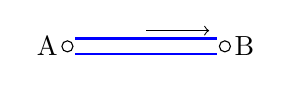
\begin{tikzpicture}
\draw (0,0) circle (2pt) node[left] {A};
\draw (2,0) circle (2pt) node[right] {B};
\draw[blue,thick] (0.1,0.1) -- (1.9,0.1);
\draw[blue,thick] (0.1,-0.1) -- (1.9,-0.1);
\draw[->] (1,0.2) -- (1.8,0.2);
\end{tikzpicture}
\caption{Pheromone trails and path selection}
\label{fig:aco_path}
\end{marginfigure}

\subsection{Differential Evolution (DE) Algorithm}
A vector-based evolutionary optimization algorithm. Provides effective results in continuous optimization problems.

\subsubsection{Basic Operators}
\begin{itemize}
    \item Mutation vector
    \item Crossover
    \item Selection
    \item Scaling factor (F)
    \item Crossover ratio (CR)
\end{itemize}

\begin{equation}
v_i = x_{r1} + F(x_{r2} - x_{r3})
\end{equation}

\begin{tcolorbox}[title=DE Strategies]
\begin{itemize}
    \item DE/rand/1/bin
    \item DE/best/1/bin
    \item DE/rand/2/bin
    \item DE/best/2/bin
    \item DE/current-to-best/1/bin
\end{itemize}
\end{tcolorbox}

\subsubsection{Algorithm Steps}
\begin{enumerate}
    \item Create initial population
    \item In each generation:
        \begin{itemize}
            \item Generate mutation vectors
            \item Apply crossover
            \item Perform selection
        \end{itemize}
    \item Continue until stopping criterion is met
\end{enumerate}

\sidenote{The differential evolution algorithm is particularly effective in continuous optimization problems. Parameter tuning is relatively easy and convergence speed is high.}

\subsection{Artificial Bee Colony (ABC) Optimization}
An optimization algorithm inspired by honey bees' food search behavior.

\subsubsection{Bee Types and Tasks}
\begin{itemize}
    \item Worker bees: Investigation of current resources
    \item Onlooker bees: Evaluation of promising resources
    \item Scout bees: Discovery of new resources
\end{itemize}

\begin{equation}
v_{ij} = x_{ij} + \phi_{ij}(x_{ij} - x_{kj})
\end{equation}

\begin{marginfigure}
\centering
\begin{tikzpicture}
\draw[->] (0,0) -- (4,0) node[right] {$x$};
\draw[->] (0,0) -- (0,4) node[above] {$f(x)$};
\filldraw[blue] (1,2) circle (2pt) node[above] {Worker};
\filldraw[red] (2,3) circle (2pt) node[above] {Onlooker};
\filldraw[green] (3,1) circle (2pt) node[above] {Scout};
\end{tikzpicture}
\caption{Role of different bee types in ABC}
\label{fig:abc_bees}
\end{marginfigure}

\subsubsection{Algorithm Steps}
\begin{enumerate}
    \item Determine initial food sources
    \item In each cycle:
        \begin{itemize}
            \item Worker bee phase
            \item Onlooker bee phase
            \item Scout bee phase
        \end{itemize}
    \item Continue until stopping criterion is met
\end{enumerate}

\subsection{Quantum and Hybrid Optimization Algorithms}
Approaches inspired by quantum mechanics principles and combining strengths of different algorithms.

\subsubsection{Quantum-Inspired Algorithms}
\begin{itemize}
    \item Quantum particle swarm
    \item Quantum genetic algorithm
    \item Quantum simulated annealing
\end{itemize}

\begin{equation}
\psi(x,t) = \frac{1}{\sqrt{2\pi\sigma^2}} e^{-\frac{(x-\mu)^2}{2\sigma^2}}
\end{equation}

\begin{tcolorbox}[title=Advantages of Quantum Mechanism]
\begin{itemize}
    \item Better exploration ability
    \item Avoiding local optima
    \item Fast convergence
    \item Utilizing uncertainty principle
\end{itemize}
\end{tcolorbox}

\subsection{Other Metaheuristic Optimization Algorithms}
Dozens of new metaheuristic optimization algorithms are added to the academic literature each year. Some of these algorithms can still present quite original approaches. However, within the basic classifications, many of them are developed by imitating certain mechanisms of previous algorithms to some extent. For an engineer looking at this topic from outside the academic perspective, understanding and being able to apply some basic algorithms is much more beneficial than constantly following new algorithms. Especially considering the development of artificial intelligence, what is really important is implementing theoretical knowledge in the right practical fields. 